\part{Introdução}

\chapter{Introdução}

Os objetivos deste capítulo são: Contextualizar o objeto de pesquisa \ref{contextualizacao}; Definir uma questão de pesquisa \ref{questao_de_pesquisa}; Justificar a necessidade da investigação \ref{justificativa}; Explanar os objetivos do presente trabalho \ref{objetivos}; E, descrever a organização dos capítulos \ref{organizacao_capitulos}. 

\section[Contextualizacao]{Contextualização}
\label{contextualizacao}

No processo de desenvolvimento de software, ainda que sejam seguidas todas as técnicas, metodologias e ferramentas previamente definidas, erros orindos em qualquer fase do produto podem acontecer \cite{maldonado_introducao_2004}. Os produtos de software que são escritos hoje, potencialmente, atinge milhões de pessoas, permitindo eles realizem trabalhos de maneira eficaz e eficiente \cite{myers2011art}. A qualidade de software continua a ser um problema e, portanto, vale considerá-la toda vez que as práticas de engenharia de software forem aplicadas. \cite{pressman_engenharia_2016}

Conforme acordado por \cite{pressman_engenharia_2016}, as principais empresas de software criam aplicações com erros (\textit{bugs}) conhecidos e os entregam a vários usuários finais. Os autores mencionam ainda que essas empresas reconhecem que as primeiras versões podem não ser da melhor qualidade, e planejam melhorias para as próximas versões.

Na década de 1990, empresas como a CIO Magazine e a Information Week informavam que eram gastos bilhões em produtos de softwares que não faziam o que deveriam fazer \cite{pressman_engenharia_2016}. Este autor ainda afima que a qualidade de software custa tempo e dinheiro, mas a falta da qualidade também tem um preço, tanto para os usuários finais como para a organização criadora.

Segundo \cite{singh2012software}, testes de software são realmente necessários para indicar os defeitos e erros que foram cometidos ao implementar produtos de software, corroborando para uma maior qualidade dos produtos gerados. Em \cite{jorgensen_software_2013}, a importância de testar é reforçada, uma vez que o autor ressalta que as implementações realizadas por programadores são passíveis de falhas. Teste de software pode ser entendido como uma investigação empírica para detectar falhas de software, bem como para que defeitos possam ser descobertos e corrigidos \cite{sommerville2011engenharia}. Dada a relevância da área de testes, ferramentas de teste costumam oferecer uma variedade de recursos, e seus usos podem reduzir significativamente os custos com testes de software \cite{sommerville2011engenharia}.

A área de testes de software é abrangente \cite{sommerville2011engenharia}, mas duas atividades destacam-se nesse contexto, sendo: verificação e validação. Ambas destinam-se a mostrar que um sistema está, respectivamente, em conformidade com a sua especificação, bem como atente às expectativas do cliente. Adicionalmente, essas atividades costumam ser tratadas em momentos diferentes do ciclo de vida de um software, conforme acordado na Figura \ref{modelo-iv-v}. Como a verificação se preocupa em avaliar se o software está de acordo com as especificações, tem-se que essa atividade ocorre desde a camada de negócios, até a construção do sistema. Já a validação, é atuante, principalmente, quando se tem um entregável funcional, permitindo a realização de testes mais avançados (Testes de Integração e Testes de Sistema), junto aos clientes ou mesmo ao público alvo. O presente trabalho procurará contribuir com a atividade de verificação, mais especificamente na fase de construção do sistema, sendo proposto um suporte para geração semi-automatizada de testes de unidade. 

\begin{figure}[h]
\centering 
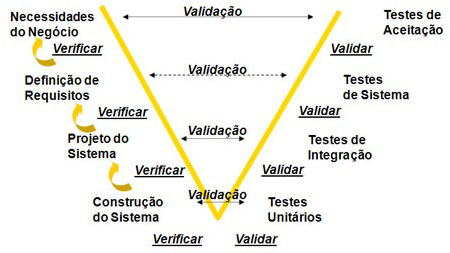
\includegraphics[width=17cm,height=10cm]{figuras/modelo-iv-v.jpg}
\caption{Modelo IV\&V.}
\label{modelo-iv-v}
\end{figure}

Como o escopo do trabalho comporta um contexto abrangente, cabem algumas considerações sobre o contexto, visando apresentar um nível maior de especificidade ao leitor. Nesse contexto, têm-se que os testadores, conforme colocado por \cite{goodliffe2007code}, estão mais preocupados com testes do tipo caixa preta. Isso significa que não se preocupam com aspectos pontuais ou mesmo mais internos (ex. casos limite e outros). O autor comenta ainda que é raro encontrar testadores que testam o código, por exemplo, no nível de produto. Por outro lado, os programadores costumam se preocupar com testes do tipo caixa branca, os quais procuram certificar que estão desenvolvendo conforme planejado. Por fim, \cite{goodliffe2007code} explica que desenvolvedores do próprio código, e que se preocupam com a atividade de testes, costumam testar de forma mais adequada do que testadores da área de qualidade (i.e. os \textit{testers} da comunidade de software). Então, o suporte a ser desenvolvido nesse trabalho pretende se orientar pela filosofia de trabalho dos programadores testadores de seus próprios códigos.

Mesmo considerando a atividade foco a de verificação; a fase de atuação a de construção de software, e a filosofia de orientação o do programador testador, o escopo do trabalho ainda seria abrangente. Dessa forma, há mais um nível de especificidade a ser considerado, no caso, o nível tecnológico. Sendo assim, o trabalho conferirá apoio a um nicho tecnológico, o qual abrange uma comunidade relevante de software Spring Boot \cite{spring_boot2019} e Jhipster \cite{jhipster2019}. Segundo um levantamento do \textit{Google Trends} houve uma busca crescente pelo termo "Spring Boot" no mundo nos últimos 5 anos, o que demonstra o interesse significativo da comunidade do Spring Boot no mundo, na Figura \ref{grafico_spring} é possível observar esse feito.

Spring Boot é um  \textit{framework} de desenvolvimento  \textit{web} bastante conhecido, e que tem como base a linguagem Java. Esse  \textit{framework} fornece um modelo de programação e de configuração \cite{gutierrez2014introducing}, procurando facilitar a criação de sistemas  \textit{stand-alone}. Aliado a esse  \textit{framework}, tem-se o \cite{jhipster2019}, um gerador de código de aplicações  \textit{web fullstack}, compatível com  Spring Boot e  Angular \cite{angular2019} \cite{raible_jhipster_2016}.

\begin{figure}[h]
\centering 
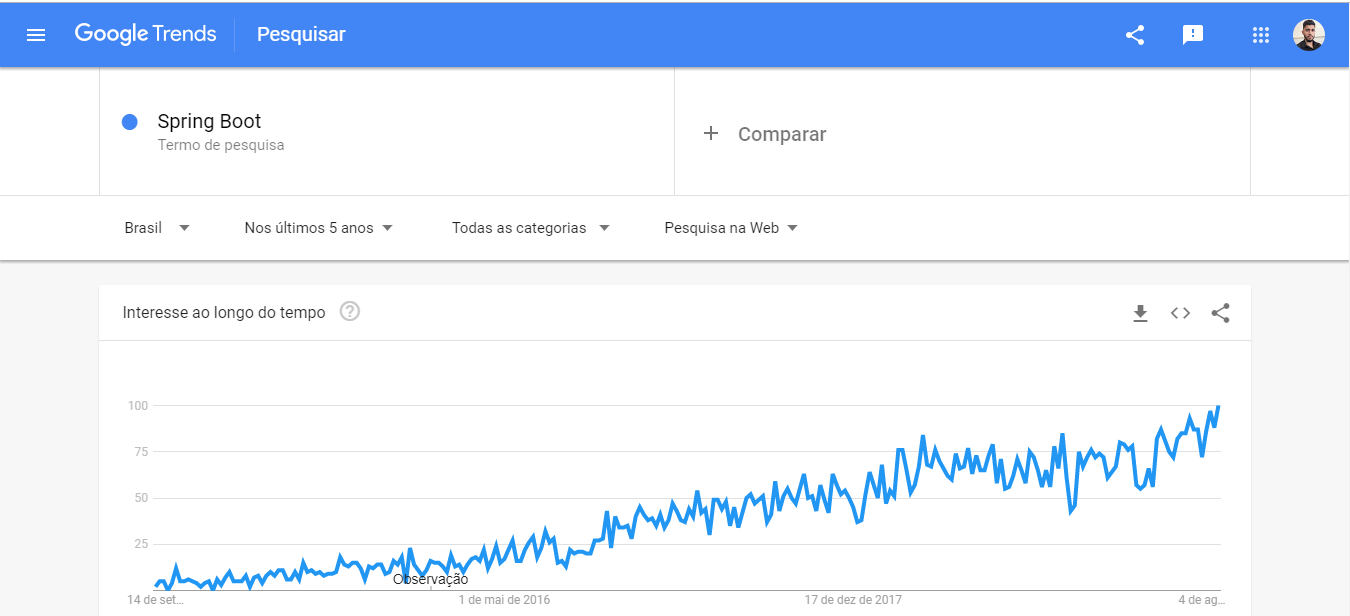
\includegraphics[width=17cm,height=10cm]{figuras/print_screen_trends.PNG}
\caption{Gráfico de Interesse do termo de pesquisa "Spring Boot" ao longo do tempo durante os últimos 5 anos.}
\label{grafico_spring}
\end{figure}

\newpage

\section[Questão de Desenvolvimento]{Questão de Desenvolvimento}
\label{questao_de_pesquisa}

Este trabalho pretende responder a seguinte questão: Como prover um suporte tecnológico semiautomatizado capaz de auxiliar desenvolvedores de produtos de software na realização de testes unitários em tempo de programação?

Lembrando que, em uma primeira versão, esse suporte será conferido em atendimento à comunidade de programadores Java, mais especificamente desenvolvedores web que se orientam pelo framework Spring Boot e pelo gerador de código web fullstack Jhipster.

\section[Justificativa]{Justificativa}
\label{justificativa}

%Uma vez que, de acordo com as investigações realizadas na literatura e na comunidade Java (vide Apêndice A para maiores detalhes), o \textit{Jhipster} gera testes de interfaces de usuário para o Angular (\textit{Protector} - http://www.protractortest.org/#/); ou ainda testes focados em \textit{JavaScript} (\textit{Jest} - https://jestjs.io/), mas, no nível de backend com Java, tem-se o uso tradicional de criação de teste unitários, com \textit{frameworks} como \textit{JUnit} e similares. Nesse último caso, cabendo aos testers de qualidade a tarefa de realizar os testes do tipo caixa preta. O presente trabalho pretende acordar um suporte semiautomatizado capaz de permitir que não apenas testers realizem tal tarefa, mas que os próprios desenvolvedores, conhecedores plenos das regras de negócio e das especificações de software, consigam realizá-la em aplicações com \textit{Spring Boot} e \textit{JHipster}, agregando valor ao produto final bem como maior qualidade ao mesmo, conforme já acordado por alguns autores \cite{goodliffe2007code}.

\section[Objetivos]{Objetivos}
\label{objetivos}

Este trabalho de conclusão de curso busca realizar o objetivo geral (Subseção \ref{objetivo_geral}) e os objetivos específicos  (Subseção \ref{objetivos_especificos}).

\subsection[Objetivo Geral]{Objetivo Geral}
\label{objetivo_geral}

Desenvolver um suporte tecnológico para geração testes unitários de forma semiautomatizada, e assim, disponilizá-lo para desenvolvedores testarem softwares em tempo de programação.

\subsection[Objetivos Específicos]{Objetivo Específicos}
\label{objetivos_especificos}
Para chegar ao objetivo final esperado é necessário realizar atividades que vão desde o conhecimento da área de testes de software até o desenvolvimento da final da ferramenta. Sendo assim, os objetivos específicos se darão da seguinte maneira:

\begin{itemize}
    \item Realizar uma revisão sistemática , a fim de acordar o referêncial teórico que embasará o projeto como um todo;
    \item Estabelecer e aplicar uma metodologia coerente com as demandas do projeto, tanto para guiar as atividades para cumprimento do TCC em si, quanto para orientar o desenvolvimento e a análise dos resultados obtidos;
    \item Desenvolver uma primeira versão do suporte visando promover a geração semiautomatizada de testes de unidade, centralizado nas tecnologias \textit{Spring Boot} e \textit{JHipster}. Esse desenvolvimento será iterativo e incremental, procurando prover, desde o TCC 1,  incrementos de software funcionais, e 
    \item Coletar resultados considerando o suporte, e revelar suas contribuições, fragilidades e possíveis melhorias. 
    
\end{itemize} 

\section[OrgCapt]{Organização dos Capitulos}
\label{organizacao_capitulos}

\begin{itemize}
    \item \textbf{Capítulo 2 Referencial Teórico:} Especifica as áreas e conceitos chaves para o desenvolvimento do trabalho;
    \item \textbf{Capítulo 3 Suporte Tecnológico:} Define as ferramentas e tecnologias que ofereceram apoio no desenvolvimento do trabalho;
    \item \textbf{Capítulo 4 Metodologia:} Explicita a metodologia utilizada na pesquisa, bem como os processos metodológicos da pesquisa;
    \item \textbf{Capítulo 5 Proposta:} Detalha a proposta em si, que é o objetivo central desse trabalho, e
    \item \textbf{Capítulo 6 Considerações Finais:} Acorda os principais resultados obtidos até o momento, com a realização do trabalho.
\end{itemize} 
